\chapter{Stationäre Wirkung und die Euler--Lagrange-Gleichung}

\lectureoverview{Der geläufige Name \emph{Prinzip der kleinsten Wirkung} verdeckt den wesentlichen Punkt: Die physikalische Bahn macht die Wirkung stationär, muss sie aber nicht minimieren. Wir werden diese Aussage ausgehend vom gewöhnlichen Gleichgewicht entwickeln, sie von Punkten auf ganze Funktionen übertragen, die Euler--Lagrange-Gleichung durch Diskretisierung einer Bahn herleiten und die Newtonschen Gleichungen wiedergewinnen. Anschließend zeigen Dreh- und Polarkoordinaten, warum die Lagrange-Formulierung mehr als eine bloße Änderung der Schreibweise ist.}

\section{Stationär, aber nicht notwendigerweise minimal}

Der unzuverlässige Teil des traditionellen Namens ist das Wort \emph{kleinsten}. Eine klassische Bahn macht die Wirkung nicht immer minimal. Im Raum der möglichen Bahnen kann sie stattdessen auch ein Maximum oder einen Sattelpunkt ergeben. Das korrekte Prinzip lautet, dass die Wirkung \emph{stationär} ist: Ihre Änderung erster Ordnung verschwindet.

Beginnen wir mit der einfacheren Frage nach dem Gleichgewicht. Ein Teilchen, das in Ruhe bleibt, hat keine Beschleunigung; folglich muss die resultierende Kraft verschwinden. Für eine Kraft, die sich aus einem eindimensionalen Potenzial ableitet, gilt
\begin{equation}
  F(x)=-\frac{dV}{dx},
  \label{eq:force-from-v}
\end{equation}
Die Gleichgewichtsbedingung lautet
\begin{equation}
  \frac{dV}{dx}=0.
  \label{eq:stationary-v-one}
\end{equation}

\begin{figure}[htbp]
  \centering
  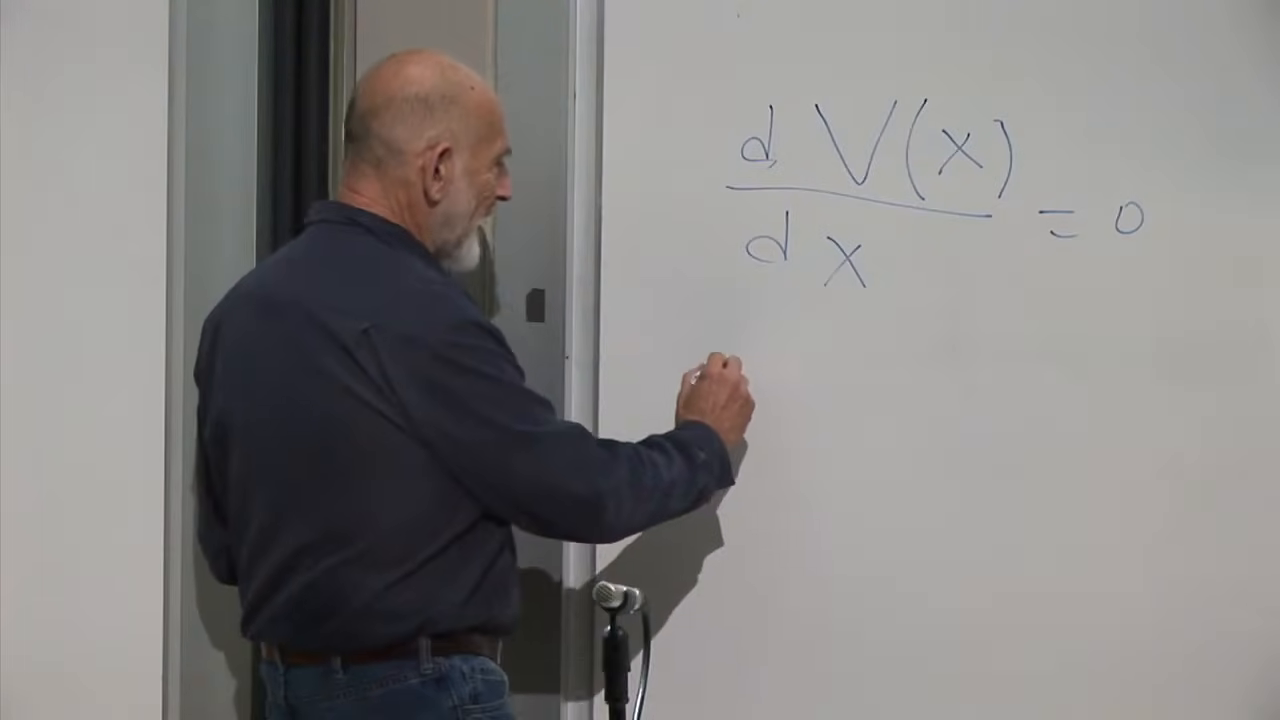
\includegraphics[width=0.74\textwidth]{lecture_03_figure_02.png}
  \caption{Die eindimensionale Gleichgewichtsbedingung: Die Kraft verschwindet dort, wo das Potenzial stationär ist.}
  \lectureframe{00:02:51}
\end{figure}

Verschieben wir das Teilchen nun um einen kleinen Betrag \(\delta x\). In erster Ordnung gilt
\begin{equation}
  \delta V
  =V(x+\delta x)-V(x)
  =\frac{dV}{dx}\,\delta x+O(\delta x^2).
  \label{eq:first-variation-one}
\end{equation}
Im Gleichgewicht verschwindet der lineare Term für beide Vorzeichen von \(\delta x\):
\begin{equation}
  \delta V=0
  \qquad\hbox{to first order.}
  \label{eq:delta-v-zero-one}
\end{equation}
Das bedeutet nicht, dass \(V\) sich nach einer endlichen Verschiebung exakt nicht ändert. Es besagt, dass die führende Änderung quadratisch oder von höherer Ordnung ist. Sowohl ein Minimum als auch ein Maximum erfüllen diese Bedingung.

\begin{figure}[htbp]
  \centering
  \begin{tikzpicture}[scale=0.95,>=Latex]
    \draw[->] (-0.2,0) -- (3.35,0) node[right] {$x$};
    \draw[->] (0,-0.2) -- (0,2.25) node[above] {$V$};
    \draw[blue!65!black,thick,smooth]
      plot coordinates {(0.2,1.85) (0.75,0.85) (1.55,0.35)
                        (2.35,0.85) (3.0,1.85)};
    \fill[red!65!black] (1.55,0.35) circle (2pt);
    \node at (1.55,-0.34) {minimum};
    \begin{scope}[xshift=4.25cm]
      \draw[->] (-0.2,0) -- (3.35,0) node[right] {$x$};
      \draw[->] (0,-0.2) -- (0,2.25) node[above] {$V$};
      \draw[blue!65!black,thick,smooth]
        plot coordinates {(0.2,0.35) (0.75,1.25) (1.55,1.85)
                          (2.35,1.25) (3.0,0.35)};
      \fill[red!65!black] (1.55,1.85) circle (2pt);
      \node at (1.55,-0.34) {maximum};
    \end{scope}
  \end{tikzpicture}
  \caption{Die Stationarität legt die erste Ableitung fest, nicht aber, ob der Punkt ein Minimum oder ein Maximum ist.}
  \label{fig:min-max-stationary}
\end{figure}

Für viele Koordinaten \(q_i\) lautet die erste Variation
\begin{equation}
  \delta V
  =\sum_i\frac{\partial V}{\partial q_i}\,\delta q_i.
  \label{eq:first-variation-many}
\end{equation}
Soll sie für jede unabhängige infinitesimale Verschiebung \(\delta q_i\) verschwinden, muss jeder Koeffizient verschwinden:
\begin{equation}
  \frac{\partial V}{\partial q_i}=0
  \qquad\hbox{for every }i.
  \label{eq:stationary-v-many}
\end{equation}

Ein zweidimensionales Potenzial stellt man sich besser als hügeliges Gelände denn als Achterbahn vor. Ein stationärer Punkt kann am Grund eines Tals, auf einem Gipfel oder an einem Sattel liegen. Am Sattel führt eine anfängliche Bewegung in eine Richtung bergauf, in einer anderen dagegen bergab. Das rücktreibende Verhalten kann daher in einer Richtung stabil und in einer anderen instabil sein, obwohl am Punkt selbst alle ersten Ableitungen verschwinden.

\begin{figure}[htbp]
  \centering
  \includegraphics[width=0.76\textwidth]{lecture_03_figure_06.png}
  \caption{Ein Sattelpunkt ist in jeder Richtung stationär in erster Ordnung, obwohl benachbarte Verschiebungen entlang der einen Achse ansteigen und entlang einer anderen abfallen.}
  \lectureframe{00:08:20}
\end{figure}

In einem Raum mit vielen Koordinaten sind Sattelpunkte typischer als reine Maxima oder Minima. Deshalb ist \emph{stationär} der treffendere Begriff. Die Bedingung
\begin{equation}
  \delta V=0
  \label{eq:equilibrium-variation}
\end{equation}
beschreibt das Gleichgewicht, ohne das Verhalten zweiter Ordnung vorwegzunehmen.

\section{Von Punkten zu Funktionen}

Die Mechanik befasst sich mit ganzen Bewegungen, nicht mit isolierten Gleichgewichtspunkten. Eine Bahn ist eine Funktion wie \(x(t)\) oder eine Sammlung von Funktionen wie \((x(t),y(t),z(t))\). Das mathematische Problem, eine Größe durch Variation einer ganzen Funktion stationär zu machen, heißt \emph{Variationsrechnung}. Bevor wir sie auf Bewegungen anwenden, betrachten wir drei einfachere Beispiele.

\subsection{Kürzeste Kurven und Geodäten}

Wir betrachten zwei feste Punkte in der Ebene und stellen eine Kurve zwischen ihnen durch \(y(x)\) dar. Für ein kurzes Kurvenstück gilt
\begin{equation}
  ds=\sqrt{dx^2+dy^2}
  =dx\sqrt{1+\left(\frac{dy}{dx}\right)^2},
  \label{eq:line-element}
\end{equation}
wobei die letzte Form \(dx>0\) voraussetzt. Die Gesamtlänge ist das Funktional
\begin{equation}
  S[y]=\int_{x_0}^{x_1}
  \sqrt{1+y'(x)^2}\,dx.
  \label{eq:arc-length-functional}
\end{equation}
Die eckigen Klammern betonen, dass \(S\) eine ganze Funktion als Eingabe erhält. Die Gerade ergibt sich aus der Bedingung
\begin{equation}
  \delta S=0
  \label{eq:stationary-length}
\end{equation}
bei kleinen Änderungen der Kurve, die beide Endpunkte festhalten.

\begin{figure}[htbp]
  \centering
  \includegraphics[width=0.78\textwidth]{lecture_03_figure_07.png}
  \caption{Eine Probekurve zwischen zwei festen Endpunkten. Ihre Länge ist die Summe der infinitesimalen Hypotenusen \(ds\).}
  \lectureframe{00:13:36}
\end{figure}

Dieselbe Frage lässt sich auf einer gekrümmten Fläche stellen. Zieht man eine Schnur zwischen zwei Pflöcken straff, erhält man ein anschauliches Bild des kürzesten Weges unter den gegebenen Einschränkungen. Eine solche Kurve mit stationärer Länge heißt \emph{Geodäte}. In einer flachen Ebene ist sie eine Gerade; auf einer Kugel oder einer hügeligen Fläche im Allgemeinen nicht.

\subsection{Fermatsches Prinzip}

Ein Lichtstrahl in einem Medium, dessen Ausbreitungsgeschwindigkeit ortsabhängig ist, \(c(x,y)\) muss nicht den räumlich kürzesten Weg nehmen. Die für ein kurzes Wegstück benötigte Zeit ist die Strecke geteilt durch die lokale Geschwindigkeit, also
\begin{equation}
  T[y]
  =\int_{x_0}^{x_1}
  \frac{\sqrt{1+y'(x)^2}}{c(x,y)}\,dx.
  \label{eq:fermat-functional}
\end{equation}
Nach dem Fermatschen Prinzip gilt
\begin{equation}
  \delta T=0.
  \label{eq:fermat-stationary}
\end{equation}
Ist \(c\) konstant, reduziert sich dies auf das Problem der kürzesten Strecke. In einem Medium mit variablem Brechungsindex gleicht der schnellste Weg dagegen die Streckenlänge und die lokale Ausbreitungsgeschwindigkeit gegeneinander ab.

\begin{figure}[htbp]
  \centering
  \includegraphics[width=0.80\textwidth]{lecture_03_figure_08.png}
  \caption{Das Funktional der Laufzeit eines Lichtstrahls in einem Medium, dessen lokale Lichtgeschwindigkeit vom Ort abhängt.}
  \lectureframe{00:22:50}
\end{figure}

Ein zeitgebundener Scherz spielt auf die damals neue Behauptung an, Neutrinos hätten sich in Italien ungewöhnlich schnell bewegt. Das physikalische Argument kehrt sofort zum verlässlichen Beispiel zurück: Gewöhnliches Licht ändert in Materie seine Geschwindigkeit entsprechend dem Brechungsindex.

\subsection{Eine hängende Kette}

Eine an zwei Punkten befestigte Kette nimmt die Form einer Kettenlinie an. Jedes kleine Stück trägt zur gravitativen potenziellen Energie bei, sodass die gesamte potenzielle Energie selbst ein Integral über die Kette ist. Wieder sind die Endpunkte fest, die unbekannte Form ist eine Funktion und ein Integral muss stationär sein.

\begin{figure}[htbp]
  \centering
  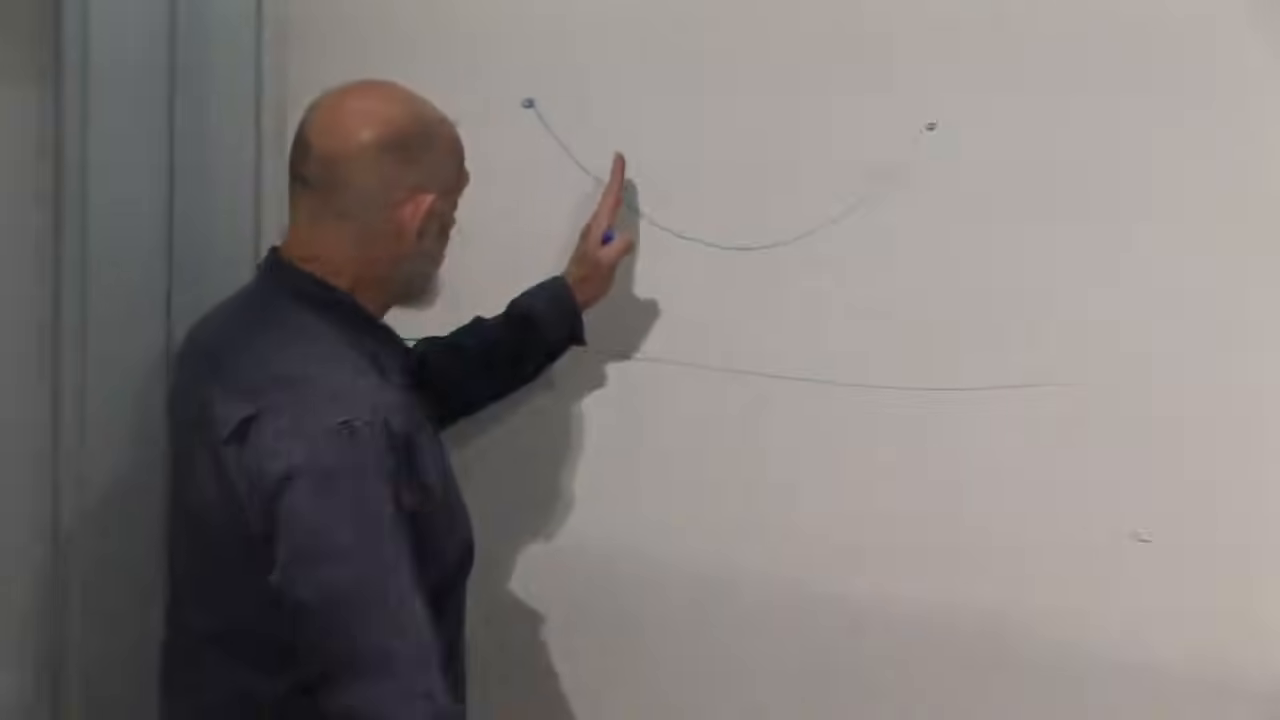
\includegraphics[width=0.76\textwidth]{lecture_03_figure_03.png}
  \caption{Eine hängende Kette zwischen festen Aufhängungen. Ihre stationäre Form wird durch die gesamte gravitative potenzielle Energie bestimmt.}
  \lectureframe{00:30:41}
\end{figure}

Diese Beispiele haben denselben Aufbau: zwei feste Endpunkte, eine Funktion zwischen ihnen und ein Integral, dessen erste Variation verschwindet. Ein solches globales Prinzip auf eine Differentialgleichung zurückzuführen, bedeutet, das Variationsproblem zu lösen.

\section{Mechanik als Randwertproblem}

Eine Bahn wird häufig mit horizontaler Zeitachse gezeichnet, weil \(t\) die unabhängige Variable ist. In der Physik gibt es dennoch die feste Konvention, die Zeit nach oben aufzutragen. Eine Randbemerkung erinnert an Experimente, bei denen Menschen Bilder von der Jugend bis ins Alter in der für ihr Schriftsystem üblichen Richtung anordneten: Leserinnen und Leser von links nach rechts ordneten sie meist von links nach rechts, Leserinnen und Leser von rechts nach links in die Gegenrichtung und vertikal Schreibende vertikal. Der Scherz schließt mit der Bemerkung, Physiker seien diejenigen, die darauf bestehen, dass die Zeit nach oben fließt. Hier verwenden wir die übliche horizontale \(t\)-Achse, weil sich \(x(t)\) so natürlich als Graph darstellen lässt.

Bei der Anfangswertformulierung lauten die Daten zum Zeitpunkt \(t_0\)
\begin{equation}
  x(t_0)=x_0,
  \qquad
  \dot x(t_0)=v_0.
  \label{eq:initial-value-data}
\end{equation}
Die Newtonsche Gleichung bestimmt dann die weitere Bahn. Eine Variationsformulierung stellt ein anderes Problem: Man gibt zwei Endereignisse vor,
\begin{equation}
  x(t_0)=x_0,
  \qquad
  x(t_1)=x_1,
  \label{eq:boundary-value-data}
\end{equation}
und bestimmt den physikalischen Weg dazwischen. Die Anfangsgeschwindigkeit wird nicht mehr vorgegeben, sondern ist Teil der Lösung.

\begin{figure}[htbp]
  \centering
  \includegraphics[width=0.76\textwidth]{lecture_03_figure_09.png}
  \caption{Eine mechanische Bahn \(x(t)\). Man kann entweder Position und Steigung an einem Ende oder die Positionen zu zwei Endzeitpunkten vorgeben.}
  \lectureframe{00:27:41}
\end{figure}

Die stationär zu machende Größe ist die \emph{Wirkung},
\begin{equation}
  A[x]=\int_{t_0}^{t_1}L(x,\dot x,t)\,dt.
  \label{eq:action-one}
\end{equation}
Der Integrand \(L\) ist die \emph{Lagrange-Funktion}. Sie kann von Ort und Geschwindigkeit sowie explizit von der Zeit abhängen. Das Wirkungsprinzip lautet
\begin{equation}
  \delta A=0
  \label{eq:stationary-action}
\end{equation}
für alle kleinen Bahnvariationen mit
\begin{equation}
  \delta x(t_0)=\delta x(t_1)=0.
  \label{eq:fixed-endpoint-variations}
\end{equation}
Die Randbedingung ist wesentlich: Verglichen werden benachbarte Bahnen, die dieselben beiden Ereignisse verbinden.

\section{Eine diskrete Herleitung der Euler--Lagrange-Gleichung}

Die Wirkung ist ein Funktional von unendlich vielen Werten der Bahn. Um ihre Variation konkret zu machen, teilen wir das Zeitintervall in Schritte der Länge \(\epsilon\) ein,
\begin{equation}
  t_n=t_0+n\epsilon,
  \qquad
  x_n=x(t_n),
  \label{eq:discrete-times}
\end{equation}
und nähern die Geschwindigkeit im \(n\)-ten Intervall an durch
\begin{equation}
  v_n=\frac{x_{n+1}-x_n}{\epsilon}.
  \label{eq:discrete-velocity}
\end{equation}
Das Integral wird damit zur gewöhnlichen Summe
\begin{equation}
  A_\epsilon
  =\sum_{n=0}^{N-1}
  \epsilon L\left(x_n,\frac{x_{n+1}-x_n}{\epsilon}\right).
  \label{eq:discrete-action}
\end{equation}
Für die Bezeichnung der Zeitschritte verwenden wir \(n\), damit \(i\) später für räumliche Koordinaten und Teilchen zur Verfügung steht.

\begin{figure}[htbp]
  \centering
  \includegraphics[width=0.82\textwidth]{lecture_03_figure_10.png}
  \caption{Die Bahn wird durch eine Kette von Zeitschritten ersetzt. Die Variation einer inneren Höhe verändert nur die beiden benachbarten Segmente.}
  \lectureframe{00:38:30}
\end{figure}

Wir variieren einen inneren Punkt \(x_n\) und halten alle übrigen \(x_k\) fest. Nur zwei Terme der Summe hängen von \(x_n\) ab:
\begin{align}
  A_\epsilon\big|_{x_n}
  &=
  \epsilon L\left(x_n,\frac{x_{n+1}-x_n}{\epsilon}\right)
  \notag\\
  &\quad+
  \epsilon L\left(x_{n-1},
                  \frac{x_n-x_{n-1}}{\epsilon}\right).
  \label{eq:two-neighbor-terms}
\end{align}
Durch Ableiten erhalten wir
\begin{align}
  0=\frac{\partial A_\epsilon}{\partial x_n}
  &=
  \epsilon\frac{\partial L_n}{\partial x_n}
  -\frac{\partial L_n}{\partial v_n}
  +\frac{\partial L_{n-1}}{\partial v_{n-1}}.
  \label{eq:discrete-el-variation}
\end{align}
Die entgegengesetzten Vorzeichen haben einen einfachen geometrischen Ursprung. Wird \(x_n\) angehoben, nimmt die Steigung des dahinterliegenden Intervalls zu und die des davorliegenden Intervalls ab.

\begin{figure}[htbp]
  \centering
  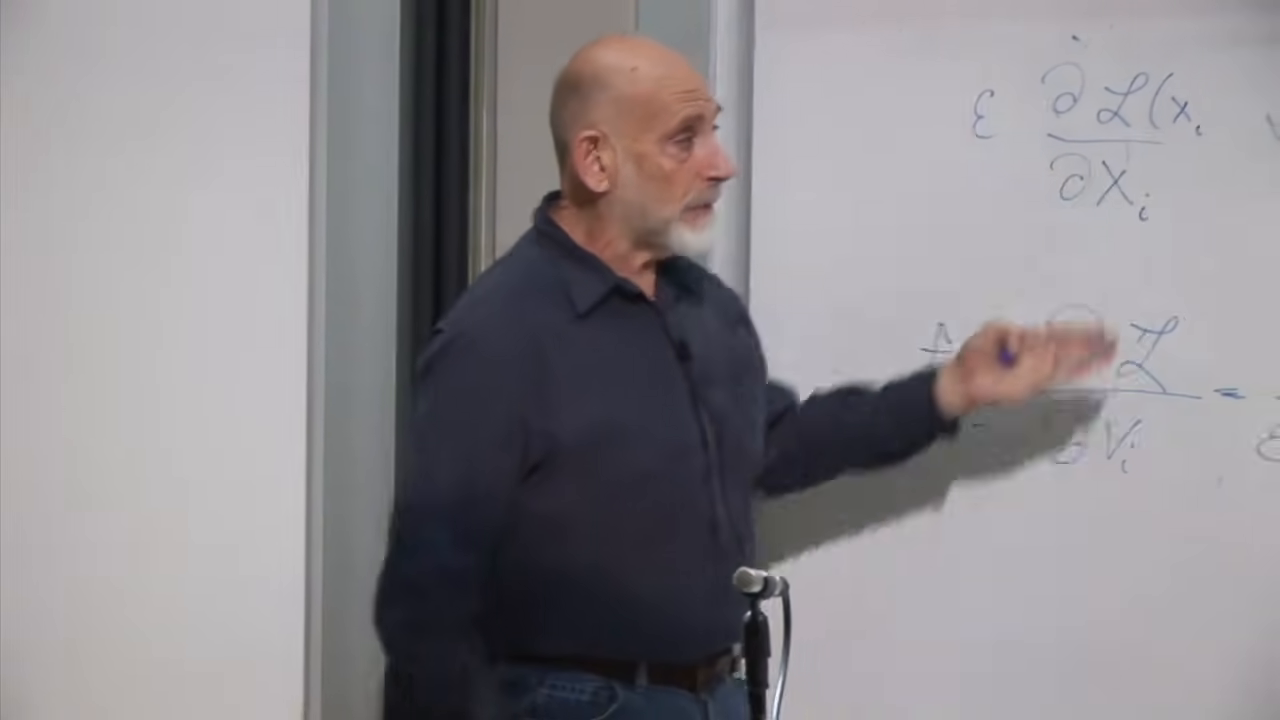
\includegraphics[width=0.74\textwidth]{lecture_03_figure_04.png}
  \caption{Der direkte Ableitungsbeitrag nach dem Ort und die beiden Beiträge der Ableitungen nach der Geschwindigkeit aus den benachbarten Intervallen bei der diskreten Variation.}
  \lectureframe{00:45:26}
\end{figure}

Stellen wir Gl.~\eqref{eq:discrete-el-variation} um:
\begin{equation}
  \frac{1}{\epsilon}
  \left(
    \frac{\partial L_n}{\partial v_n}
    -\frac{\partial L_{n-1}}{\partial v_{n-1}}
  \right)
  =
  \frac{\partial L_n}{\partial x_n}.
  \label{eq:discrete-el}
\end{equation}
Die linke Seite ist ein Differenzenquotient benachbarter Werte. Für \(\epsilon\to0\) wird aus der gebrochenen Linie eine glatte Bahn und der Quotient eine Zeitableitung:
\begin{equation}
  \boxed{
  \frac{d}{dt}\left(\frac{\partial L}{\partial\dot x}\right)
  =
  \frac{\partial L}{\partial x}}
  .
  \label{eq:euler-lagrange-one}
\end{equation}
Dies ist die Euler--Lagrange-Gleichung.

\begin{figure}[htbp]
  \centering
  \includegraphics[width=0.78\textwidth]{lecture_03_figure_11.png}
  \caption{Die vollständige Euler--Lagrange-Gleichung, die sich aus der Stationarität an jedem inneren Zeitschritt ergibt.}
  \lectureframe{00:49:25}
\end{figure}

Sobald \(L\) festgelegt ist, funktioniert Gl.~\eqref{eq:euler-lagrange-one} wie eine Rechenvorschrift: Man leitet die gegebene Funktion ab und erhält eine Differentialgleichung für die Bahn.

\begin{classroomqa}\audiencequestion{Gilt das Ergebnis von Euler--Lagrange für jede Funktion von \(x\) und \(\dot x\)?\lecturetimestamp{00:49:37--00:50:24}}\lecturerresponse{Ja, sofern die für die Ableitungen erforderliche Regularität gegeben ist. Beim Beispiel der Bogenlänge erhält man genau dieselbe Form, wenn man die unabhängige Variable \(x\) der Rolle von \(t\) und die gesuchte Funktion \(y(x)\) der Rolle von \(x(t)\) zuordnet. Die Lösungen der zugehörigen Euler--Lagrange-Gleichung sind Geraden.}\end{classroomqa}

\section{Newtons Gleichungen aus der Lagrange-Funktion}

Für ein Teilchen auf einer Geraden im Potenzial \(V(x)\) wählen wir
\begin{equation}
  L(x,\dot x)=T-V
  =\frac12m\dot x^2-V(x).
  \label{eq:lagrangian-tv-one}
\end{equation}
Das Minuszeichen mag seltsam erscheinen, weil die Gesamtenergie \(T+V\) ist. Doch die Lagrange-Funktion ist nicht die Energie. Entscheidend ist, ob die Euler--Lagrange-Vorschrift die richtige Bewegung ergibt. Eine scherzhafte Abstimmung über das Vorzeichen wird abgelehnt: Die Antwort muss überprüft, nicht gewählt werden.

Zunächst gilt
\begin{equation}
  \frac{\partial L}{\partial\dot x}=m\dot x.
  \label{eq:conjugate-momentum-one}
\end{equation}
Dies ist der Impuls. Allgemeiner ist der einer beliebigen Koordinate \(q\) konjugierte Impuls definiert durch
\begin{equation}
  p_q=\frac{\partial L}{\partial\dot q}.
  \label{eq:conjugate-momentum-general}
\end{equation}
Die Zeitableitung von Gl.~\eqref{eq:conjugate-momentum-one} ergibt \(m\ddot x\), während
\begin{equation}
  \frac{\partial L}{\partial x}
  =-\frac{dV}{dx}.
  \label{eq:lagrangian-position-derivative}
\end{equation}
Damit lautet die Euler--Lagrange-Gleichung
\begin{equation}
  m\ddot x=-\frac{dV}{dx}=F(x),
  \label{eq:newton-from-action}
\end{equation}
also das zweite Newtonsche Gesetz.

\begin{figure}[htbp]
  \centering
  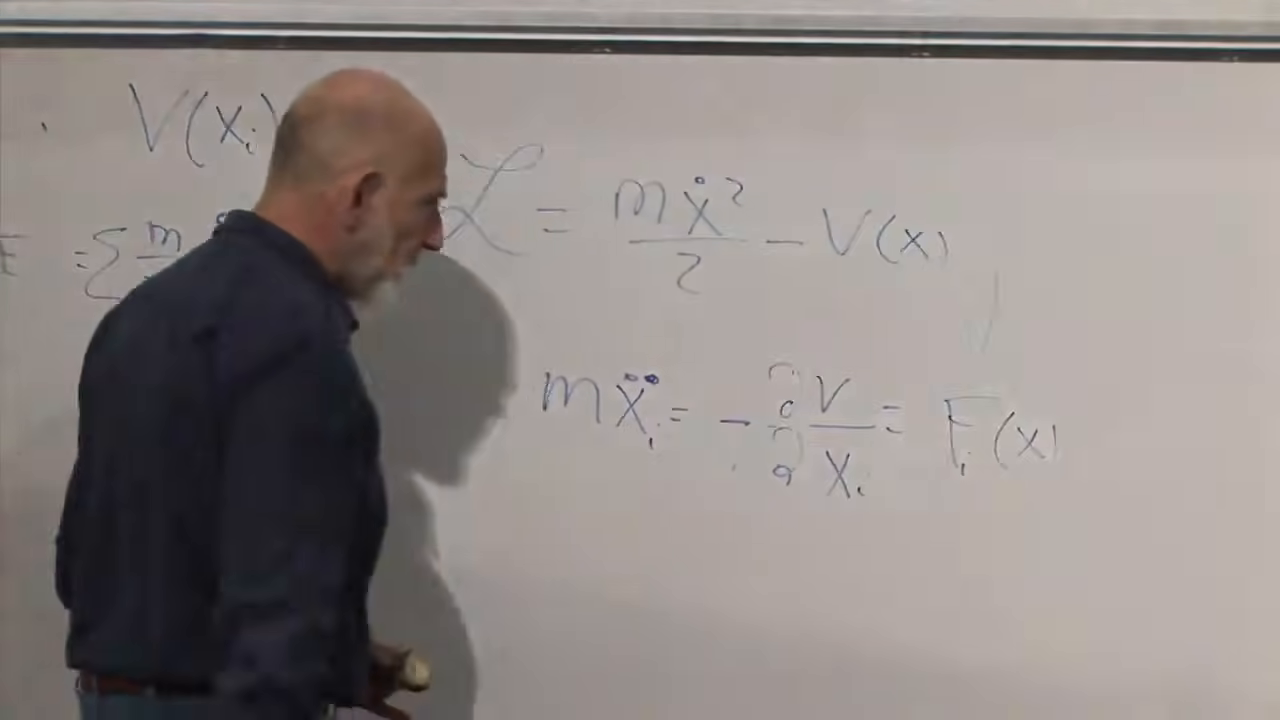
\includegraphics[width=0.80\textwidth]{lecture_03_figure_05.png}
  \caption{Kinetische Energie, potenzielle Energie, \(L=T-V\) und die wiedergewonnene Komponentenform der Newtonschen Gleichung an einer Tafel.}
  \lectureframe{00:57:52}
\end{figure}

Für viele Koordinaten \(q_i\) gilt
\begin{equation}
  L(\mathbf q,\dot{\mathbf q})
  =\sum_i\frac12m_i\dot q_i^{\,2}-V(q_1,q_2,\ldots),
  \label{eq:lagrangian-tv-many}
\end{equation}
und für jede Koordinate gibt es eine Gleichung:
\begin{equation}
  \frac{d}{dt}\left(\frac{\partial L}{\partial\dot q_i}\right)
  =\frac{\partial L}{\partial q_i}
  \quad\Longrightarrow\quad
  m_i\ddot q_i=-\frac{\partial V}{\partial q_i}=F_i.
  \label{eq:euler-lagrange-many}
\end{equation}
Die Bahn bleibt eine einzige Kurve, verläuft nun aber durch einen hochdimensionalen Konfigurationsraum.

\begin{classroomqa}\audiencequestion{Sind wir nicht einfach vom Newtonschen Gesetz rückwärts ausgegangen und haben ein Funktional so konstruiert, dass es das Ergebnis reproduziert?\lecturetimestamp{00:58:07--01:00:04}}\lecturerresponse{Das ist keine zielführende Sichtweise. Die Lagrange-Funktion ist die kompakte Beschreibung des physikalischen Systems: Eine Funktion aller Koordinaten und Geschwindigkeiten fasst sämtliche Bewegungsgleichungen zusammen. Bei neuen Theorien schlagen Physiker gewöhnlich eine Wirkung vor und leiten daraus die Gleichungen her, statt jede Gleichung einzeln zu erraten.}\end{classroomqa}

Diese Zusammenfassung ist ein Vorteil. Die Freiheit der Koordinaten ist ein weiterer. Die Aussage, dass eine Linie die kürzeste ist, hängt nicht davon ab, ob die Ebene mit kartesischen, polaren oder krummlinigen Koordinaten beschrieben wird. Ebenso ist die Stationarität der Wirkung koordinatenunabhängig, auch wenn sich die Formel für \(L\) und die daraus folgenden Komponentengleichungen ändern.

\section{Ein freies Teilchen vom Karussell aus gesehen}

Seien \((x,y)\) inertiale kartesische Koordinaten und \((X,Y)\) kartesische Koordinaten, die sich gleichförmig mit der Winkelgeschwindigkeit \(\omega\) drehen. Bei der hier verwendeten Orientierung gilt
\begin{align}
  x&=X\cos\omega t+Y\sin\omega t,
  \notag\\
  y&=-X\sin\omega t+Y\cos\omega t.
  \label{eq:rotating-coordinate-map}
\end{align}
Der Winkel zwischen den Bezugssystemen beträgt \(\omega t\).

\begin{figure}[htbp]
  \centering
  \includegraphics[width=0.76\textwidth]{lecture_03_figure_12.png}
  \caption{Inertiale und gleichförmig rotierende kartesische Achsen. Derselbe Punkt erhält zeitabhängige rotierende Koordinaten.}
  \lectureframe{01:06:05}
\end{figure}

Die Lagrange-Funktion eines freien Teilchens im Inertialsystem lautet
\begin{equation}
  L_{\mathrm{in}}
  =\frac{m}{2}\left(\dot x^2+\dot y^2\right).
  \label{eq:free-inertial-lagrangian}
\end{equation}
Leiten wir Gl.~\eqref{eq:rotating-coordinate-map} ab und verwenden \(\sin^2\omega t+\cos^2\omega t=1\). Die trigonometrischen Terme lassen sich zusammenfassen zu
\begin{align}
  \dot x^2+\dot y^2
  &=
  \dot X^2+\dot Y^2\\
  &\quad+\omega^2(X^2+Y^2)\\
  &\quad+2\omega(Y\dot X-X\dot Y).
  \label{eq:rotating-speed}
\end{align}
Somit gilt
\begin{align}
  L_{\mathrm{rot}}
  &=
  \frac{m}{2}(\dot X^2+\dot Y^2)\\
  &\quad+\frac{m\omega^2}{2}(X^2+Y^2)\\
  &\quad+m\omega(Y\dot X-X\dot Y).
  \label{eq:rotating-lagrangian}
\end{align}

\begin{figure}[htbp]
  \centering
  \includegraphics[width=0.84\textwidth]{lecture_03_figure_13.png}
  \caption{Die transformierte Lagrange-Funktion des freien Teilchens: gewöhnliche kinetische Energie, ein quadratischer Zentrifugalterm und ein linearer Geschwindigkeitsterm.}
  \lectureframe{01:12:16}
\end{figure}

Der quadratische Koordinatenterm hat die Form \(-V_{\mathrm{fict}}\), wobei
\begin{equation}
  V_{\mathrm{fict}}
  =-\frac{m\omega^2}{2}(X^2+Y^2).
  \label{eq:centrifugal-potential}
\end{equation}
Das entsprechende Potenzial nimmt nach außen hin ab und erzeugt daher die Zentrifugalkraft \(m\omega^2(X,Y)\).

Der letzte Term in Gl.~\eqref{eq:rotating-lagrangian} ist sowohl in den Koordinaten als auch in den Geschwindigkeiten linear. Die Euler--Lagrange-Gleichung liefert
\begin{align}
  m\ddot X&=m\omega^2X-2m\omega\dot Y,
  \notag\\
  m\ddot Y&=m\omega^2Y+2m\omega\dot X.
  \label{eq:rotating-equations}
\end{align}
Die Terme proportional zu \(\omega^2\) sind Zentrifugalterme; die geschwindigkeitsproportionalen Terme sind Coriolis-Terme. In Vektorform innerhalb der rotierenden Ebene gilt
\begin{equation}
  \mathbf F_{\mathrm{C}}
  =-2m\,\boldsymbol\omega\times\mathbf v_{\mathrm{rot}},
  \label{eq:coriolis-vector}
\end{equation}
wobei sich die Vorzeichen ändern, wenn die entgegengesetzte Orientierungskonvention verwendet wird.

\begin{figure}[htbp]
  \centering
  \includegraphics[width=0.84\textwidth]{lecture_03_figure_14.png}
  \caption{Die Gleichungen im rotierenden Bezugssystem: Die koordinatenproportionalen Terme liefern Zentrifugalbeschleunigungen, die geschwindigkeitsabhängigen Kreuzterme Coriolisbeschleunigungen.}
  \lectureframe{01:20:20}
\end{figure}

Der Punkt ist nicht, dass die Algebra wegfällt. Vielmehr erzeugt eine einzige Koordinatentransformation einer einzelnen skalaren Funktion beide gekoppelten Gleichungen und beide Scheinkräfte.

\begin{classroomqa}\audiencequestion{Funktioniert diese Methode auch für beliebig gekrümmte Koordinaten?\lecturetimestamp{01:22:01--01:22:17}}\lecturerresponse{Ja. Die neuen Koordinaten können krummlinig sein und sogar explizit von der Zeit abhängen, wie es bei den rotierenden Koordinaten der Fall ist. Man schreibt die Wirkung in den neuen Variablen um und wendet dieselbe Euler--Lagrange-Regel an.}\end{classroomqa}

\section{Polarkoordinaten und ein zyklischer Winkel}

Für gewöhnliche Polarkoordinaten gilt
\begin{equation}
  x=r\cos\theta,
  \qquad
  y=r\sin\theta.
  \label{eq:polar-map}
\end{equation}
Sowohl \(r\) als auch \(\theta\) können sich mit der Zeit ändern. Ableiten und Quadrieren der Komponenten sowie anschließendes Addieren ergibt
\begin{equation}
  \dot x^2+\dot y^2
  =\dot r^2+r^2\dot\theta^2.
  \label{eq:polar-speed}
\end{equation}
Für ein Zentralpotenzial \(V(r)\) lautet die Lagrange-Funktion
\begin{equation}
  L
  =\frac{m}{2}\left(\dot r^2+r^2\dot\theta^2\right)-V(r).
  \label{eq:polar-lagrangian}
\end{equation}

\begin{figure}[htbp]
  \centering
  \includegraphics[width=0.80\textwidth]{lecture_03_figure_15.png}
  \caption{Polargeometrie und die Zerlegung der kinetischen Energie in Radial- und Winkelbewegung.}
  \lectureframe{01:23:30}
\end{figure}

Die Radialgleichung lautet
\begin{equation}
  m\ddot r
  =mr\dot\theta^2-\frac{dV}{dr}.
  \label{eq:radial-equation}
\end{equation}
Der erste Term ist der nach außen gerichtete Zentrifugalbeitrag, der mit der Winkelbewegung des Teilchens selbst zusammenhängt.

Für den Winkel gilt
\begin{equation}
  \frac{d}{dt}\left(\frac{\partial L}{\partial\dot\theta}\right)
  =\frac{\partial L}{\partial\theta}=0,
  \label{eq:theta-el}
\end{equation}
weil das Zentralpotenzial keine explizite Abhängigkeit von \(\theta\) hat. Daher gilt
\begin{equation}
  \frac{d}{dt}\left(mr^2\dot\theta\right)=0,
  \qquad
  mr^2\dot\theta=\ell,
  \label{eq:angular-momentum}
\end{equation}
wobei \(\ell\) der erhaltene Drehimpuls ist.

\begin{figure}[htbp]
  \centering
  \includegraphics[width=0.82\textwidth]{lecture_03_figure_16.png}
  \caption{Die Euler--Lagrange-Gleichung für den Winkel hat eine rechte Seite von null und macht so die Erhaltung von \(mr^2\dot\theta\) sichtbar.}
  \lectureframe{01:29:25}
\end{figure}

Die Winkelgleichung ergibt
\begin{equation}
  \dot\theta=\frac{\ell}{mr^2}.
  \label{eq:theta-dot-angular-momentum}
\end{equation}
Einsetzen in Gl.~\eqref{eq:radial-equation} lässt eine einzige Gleichung für \(r\) übrig:
\begin{equation}
  m\ddot r
  =\frac{\ell^2}{mr^3}-\frac{dV}{dr}.
  \label{eq:effective-radial-equation}
\end{equation}

Eine in \(L\) nicht vorkommende Koordinate heißt traditionell \emph{zyklisch}, selbst wenn sie kein Winkel ist. Ist \(q\) zyklisch, gilt
\begin{equation}
  \frac{\partial L}{\partial q}=0
  \quad\Longrightarrow\quad
  \frac{d}{dt}\left(\frac{\partial L}{\partial\dot q}\right)=0.
  \label{eq:cyclic-conservation}
\end{equation}
Ihr konjugierter Impuls ist erhalten. Dies ist ein erster Hinweis auf den allgemeinen Zusammenhang zwischen Symmetrie und Erhaltungssatz.

\section{Fragen zu Bedeutung, Energie und Geltungsbereich}

Die folgenden Fragen machen deutlich, worin der tiefere Gehalt des Formalismus liegt.

\begin{classroomqa}\audiencequestion{Gibt es neben der Erkenntnis, dass die Lagrange-Funktion die richtigen klassischen Gleichungen liefert, einen unabhängigen Grund, auf sie zu kommen?\lecturetimestamp{01:33:25--01:35:07}}\lecturerresponse{Historisch zeigte sich im Verlauf von mehr als einem Jahrhundert klassischer Mechanik, dass sich Teilchen, Wellen und elektromagnetische Felder alle in dieser Form darstellen lassen. Auf der klassischen Ebene ist dieser anhaltende Erfolg eine empirische Tatsache darüber, wie physikalische Gesetze strukturiert sind. Die tiefere Erklärung stammt aus der Quantenmechanik und wird später behandelt.}\end{classroomqa}

\begin{classroomqa}\audiencequestion{Lässt sich dem geschwindigkeitslinearen Term in der Lagrange-Funktion des rotierenden Bezugssystems eine gewöhnliche kinetische oder potenzielle Energie zuordnen?\lecturetimestamp{01:35:08--01:36:23}}\lecturerresponse{Nein. Die zur Zeittranslation gehörende erhaltene Größe erhält man durch die Hamilton-Konstruktion und nicht dadurch, dass man jeden Term in \(L\) als kinetische oder potenzielle Energie deutet. Bei Gl.~\eqref{eq:rotating-lagrangian} hebt sich der geschwindigkeitslineare Term in \(\sum_a\dot q_a\,\partial L/\partial\dot q_a-L\) auf. Die Hamilton-Behandlung wird dies systematisch ordnen.}\end{classroomqa}

Da \(L_{\mathrm{rot}}\) tatsächlich nicht explizit von der Zeit abhängt, ist
\begin{equation}
  \begin{aligned}
    H_{\mathrm{rot}}
    &=\dot X\frac{\partial L}{\partial\dot X}
     +\dot Y\frac{\partial L}{\partial\dot Y}-L\\
    &=\frac{m}{2}(\dot X^2+\dot Y^2)
     -\frac{m\omega^2}{2}(X^2+Y^2)
  \end{aligned}
  \label{eq:rotating-hamiltonian-preview}
\end{equation}
erhalten. Dies ist das Jacobi-Integral im rotierenden Bezugssystem, nicht dieselbe numerische Energie, die ein Inertialbeobachter angibt. Zeitabhängige Koordinatenwechsel müssen die numerische Form der Energie nicht erhalten.

\begin{classroomqa}\audiencequestion{Was ist, wenn eine gekrümmte Bahn durch die Gravitation verursacht wird?\lecturetimestamp{01:36:30--01:37:10}}\lecturerresponse{Für die Newtonsche Gravitation setzt man einfach \(V(r)=-GMm/r\) in die Lagrange-Funktion für ein Zentralfeld ein. Gekrümmte Raumzeit gehört zur allgemeinen Relativitätstheorie und wird hier nicht vorausgesetzt.}\end{classroomqa}

\begin{classroomqa}\audiencequestion{Sind das Zentrifugalpotenzial und seine Energie lediglich fiktiv?\lecturetimestamp{01:37:13--01:40:14}}\lecturerresponse{Ein Beobachter auf der rotierenden Plattform misst die effektiven Kräfte und kann die erhaltene Größe im rotierenden Bezugssystem widerspruchsfrei verwenden. \emph{Fiktiv} bedeutet, dass diese Terme aus einer nichtinertialen Beschreibung hervorgehen, nicht, dass ihre beobachteten Wirkungen eingebildet wären. Die Energie selbst ist unter einem allgemeinen zeitabhängigen Koordinatenwechsel nicht invariant.}\end{classroomqa}

\begin{classroomqa}\audiencequestion{In welche Richtung zeigt die geschwindigkeitsabhängige Corioliskraft?\lecturetimestamp{01:40:22--01:42:36}}\lecturerresponse{Sie steht senkrecht auf der Geschwindigkeit im rotierenden Bezugssystem; ihr Betrag ist proportional zur Geschwindigkeit und zur Winkelgeschwindigkeit des Bezugssystems. In der Ebene werden die Komponenten \(\dot X\) und \(\dot Y\) mit entgegengesetzten Vorzeichen vertauscht, wie in Gl.~\eqref{eq:rotating-equations}.}\end{classroomqa}

\begin{figure}[htbp]
  \centering
  \includegraphics[width=0.76\textwidth]{lecture_03_figure_17.png}
  \caption{Das Muster der gekreuzten Geschwindigkeitskomponenten: Die Corioliskraft steht senkrecht auf der Geschwindigkeit im rotierenden Bezugssystem.}
  \lectureframe{01:41:40}
\end{figure}

\begin{classroomqa}\audiencequestion{Muss die Ausgangs-Lagrange-Funktion in einem Inertialsystem formuliert sein?\lecturetimestamp{01:42:37--01:44:00}}\lecturerresponse{Für ein gewöhnliches freies Teilchen liefert das Newtonsche Trägheitsgesetz im Inertialsystem die einfache Ausgangsform \(m(\dot x^2+\dot y^2)/2\). Sobald dieses physikalische Gesetz bekannt ist, lässt sich die Wirkung in beliebige andere Koordinaten transformieren. Man sollte nicht unabhängig davon dieselbe einfache kinetische Formel in einem rotierenden Bezugssystem voraussetzen.}\end{classroomqa}

Dieselbe Art geschwindigkeitslinearen Term gibt es bei einem geladenen Teilchen in einem Magnetfeld:
\begin{equation}
  L_{\mathrm{em}}
  =\frac12m\mathbf v^2
   +q\mathbf A(\mathbf r,t)\cdot\mathbf v
   -q\phi(\mathbf r,t).
  \label{eq:electromagnetic-lagrangian}
\end{equation}
Für ein homogenes Magnetfeld senkrecht zur Ebene liefert die symmetrische Eichung \(\mathbf A=\tfrac12\mathbf B\times\mathbf r\) einen Term proportional zu \(X\dot Y-Y\dot X\), der dieselbe algebraische Struktur wie der Coriolisterm hat.

\begin{figure}[htbp]
  \centering
  \includegraphics[width=0.82\textwidth]{lecture_03_figure_18.png}
  \caption{Der geschwindigkeitslineare Term in der Lagrange-Funktion des rotierenden Bezugssystems, der den Vergleich mit einem geladenen Teilchen in einem homogenen Magnetfeld nahelegt.}
  \lectureframe{01:44:40}
\end{figure}

\begin{classroomqa}\audiencequestion{Gibt es über die Glattheit hinaus Einschränkungen dafür, welche Funktion als Lagrange-Funktion dienen kann?\lecturetimestamp{01:44:46--01:45:06}}\lecturerresponse{Ja, aber die relevanten Einschränkungen setzen mehr voraus, als wir bisher entwickelt haben, und werden später behandelt. Die zentrale Erkenntnis an dieser Stelle ist, wie eine vorgeschlagene Lagrange-Funktion Gleichungen und Erhaltungssätze erzeugt.}\end{classroomqa}

Die Gleichungen im rotierenden Bezugssystem lassen auch Kreisbewegungen zu: Ein im Inertialsystem ruhender Punkt erscheint vom Karussell aus gesehen auf einem Kreis um den rotierenden Ursprung. Die Analogie zum Magnetfeld erklärt dann, warum ein geladenes Teilchen eine kreisförmige Zyklotronbewegung ausführen kann.

\begin{classroomqa}\audiencequestion{Bliebe ein geladenes Teilchen auf dieser Kreisbahn, oder würde die Strahlung die Bahn zum Kollaps bringen?\lecturetimestamp{01:46:11--01:47:21}}\lecturerresponse{Die hier betrachteten Gleichungen für das Teilchen allein berücksichtigen keine Strahlung. Bezieht man die Kopplung an das elektromagnetische Feld und die Strahlungsrückwirkung ein, kann eine beschleunigte klassische Ladung Strahlung aussenden. Die Strahlung ist somit ein zusätzlicher physikalischer Effekt und kein Widerspruch zur Bahn in den vereinfachten Gleichungen.}\end{classroomqa}

\begin{classroomqa}\audiencequestion{Welche Rolle spielen Hurrikane in dieser Diskussion?\lecturetimestamp{01:47:30--01:47:50}}\lecturerresponse{Die großräumige Bewegung der Atmosphäre findet auf der rotierenden Erde statt; daher sind Corioliseffekte wichtig. Eine angemessene Herleitung gehört in die Meteorologie und wird hier nicht versucht.}\end{classroomqa}

\begin{classroomqa}\audiencequestion{Soll der Wirkungsformalismus jedes physikalische Gesetz erfassen, und was würde eine echte Ausnahme bedeuten?\lecturetimestamp{01:47:57--01:49:01}}\lecturerresponse{Jede bekannte abgeschlossene fundamentale Theorie im hier betrachteten Rahmen lässt sich durch eine Wirkung beschreiben: Newtonsche Teilchen, Maxwell-Felder, allgemeine Relativitätstheorie und das Standardmodell. Scheinbare Gegenbeispiele wie viskose Reibung entstehen, wenn Freiheitsgrade der Umgebung weggelassen werden. Bezieht man das Fluid oder das mikroskopische Wärmebad in das System ein, fügt sich die fundamentale Beschreibung wieder in diesen Rahmen. Eine wirklich fundamentale Ausnahme wäre daher eine bedeutende Entdeckung.}
\end{classroomqa}